\documentclass[11pt, letterpaper]{article}
\setlength{\parindent}{0in}
\setlength{\textheight}{8.7in}
\setlength{\textwidth}{6.8in}
\setlength{\oddsidemargin}{-0.3in}
\setlength{\evensidemargin}{0.0in}
\addtolength{\topmargin}{-1in}
\setlength{\parskip}{0.1in}

\usepackage{amsmath, amsfonts, amssymb, color}
\usepackage{bm}
\usepackage{booktabs}
\usepackage{enumerate}
\usepackage{graphicx}
\usepackage{pdfpages}
\newcommand*{\justifyheading}{\raggedleft}


\renewcommand{\baselinestretch}{1.0}

\newcommand{\bx}{{\bm x}}
\newcommand{\bX}{{\bm X}}
\newcommand{\by}{{\bm y}}
\newcommand{\bY}{{\bm Y}}
\newcommand{\bW}{{\bm W}}
\newcommand{\bG}{{\bm G}}
\newcommand{\bR}{{\bm R}}
\newcommand{\bZ}{{\bm Z}}
\newcommand{\bV}{{\bm V}}
\newcommand{\bL}{{\bm L}}
\newcommand{\bz}{{\bm z}}
\newcommand{\be}{{\bm e}}
\newcommand{\bgamma}{{\bm \gamma}}
\newcommand{\bbeta}{{\bm \beta}}
\newcommand{\balpha}{{\bm \alpha}}
\newcommand{\bSigma}{{\bm \Sigma}}
\newcommand{\bmu}{{\bm \mu}}
\newcommand{\btheta}{{\bm \theta}}
\newcommand{\bepsilon}{{\bm \epsilon}}
\newcommand{\bone}{{\bm 1}}
\newcommand{\bzero}{{\bm 0}}
\newcommand{\bC}{{\bm C}}
\newcommand{\bI}{{\bm I}}
\newcommand{\bA}{{\bm A}}
\newcommand{\bB}{{\bm B}}
\newcommand{\bQ}{{\bm Q}}
\newcommand{\bS}{{\bm S}}
\newcommand{\bD}{{\bm D}}
\newcommand{\cQ}{\mathcal{Q}}
\newcommand{\cU}{\mathcal{U}}
\newcommand{\cI}{\mathcal{I}}
\newcommand{\cL}{\mathcal{L}}

\newcommand{\beas}{\begin{eqnarray*}}
\newcommand{\eeas}{\end{eqnarray*}}

\newenvironment{equationarrayright}{
                          \begin{eqnarray*}
                          \begin{array}{rcll}
                         }{
                          \end{array}
                          \end{eqnarray*}
                         }
\newcommand{\bear}{\begin{equationarrayright}}
\newcommand{\eear}{\end{equationarrayright}}

\renewcommand\arraystretch{1.3}

\DeclareMathOperator*{\argmin}{arg\,min}

\title{STAT/BIOST 571: Homework 4}
\author{Philip Pham}
\date{\today}

\begin{document}

\maketitle

\section*{Problem 1: Iterative methods for solving GEE (10 points)} 

{\em In this problem, you will compare
variants on GEE (or general linear model) estimation procedures when applied to the example dental data set for the model on slide 2.71.
Throughout, use a homoscedastic AR-1 working covariance matrix and estimate $\alpha$ and $\sigma^2$
using moment-based estimators.
For each procedure, compute point estimates and robust sandwich-based standard errors that account for clustering.  Where applicable, report how many interations are required to get convergence of all estimates 
($\bbeta$, $\alpha$, and $\sigma^2$) in their 1st/2nd/3rd significant figures.}
\begin{enumerate}[(a)]
{\em \item Use the non-iterative procedure we have employed previously; that is, first estimate $\bbeta$ by OLS, then estimate the covariance parameters based on residuals from the OLS fit, and then restimate $\bbeta$ 
  using the updated working covariance matrix. }

\begin{description}
\item[Solution:] The covariance structure for each cluster $i$ is assumed to be
  the $m_i \times m_i$ matrix $\Sigma_i$, where $\Sigma_{ijj} = \sigma^2$ and
  $\Sigma_{ijk} = \sigma^2\alpha^{\left\lvert j - k\right\rvert}$.

  Given a working estimate of $\beta$, say $\hat{\beta}^{(t)}$, we compute
  working covariance matrices for each cluster
  \[\hat{\Sigma}_i^{(t + 1)} = \left(y_i - X_i\hat{\beta}^{(t)}\right)\left(y_i -
      X_i\hat{\beta}^{(t)}\right)^\intercal.\] We get working estimates of the
  covariance parameters $\alpha$ and $\sigma^2$:
  \begin{align*}
    \left(\hat{\sigma}^2\right)^{(t + 1)}
    &= \frac{1}{\sum_{i=1}^nm_i}\sum_{i=1}^n\sum_{j=1}^{m_i}\hat{\Sigma}_{ijj}^{(t + 1)} \\
    \hat{\alpha}^{(t + 1)}
    &= \frac{1}{\left(\hat{\sigma}^2\right)^{(t + 1)}\sum_{i=1}^n\left(m_i - 1\right)}
      \sum_{i=1}^n\sum_{j=1}^{m_i-1}\hat{\Sigma}_{i,j,j+1}^{(t + 1)}.
  \end{align*}


  Let $\hat{V}^{(t+1)}$ be the matrix where
  $\hat{V}_{ij}^{(t+1)} = \left(\hat{\sigma}^2\right)^{(t+1)}
  \left(\hat{\alpha}^{(t+1)}\right)^{\lvert j - i\rvert}$. Let
  $\hat{W}^{(t+1)} = \left(\hat{V}^{(t+1)}\right)^{-1}$.

  Then, we
  can get an updated estimate of $\beta$:
  \begin{equation}
    \hat{\beta}^{(t+1)} =
    \left(
      \sum_{i=1}^n X_i^\intercal \hat{W}^{(t+1)} X_i
    \right)^{-1}
    \left(
      \sum_{i=1}^n X_i^\intercal \hat{W}^{(t+1)} y_i
    \right).
  \end{equation}

  We can compute the covariance of this estimate with the sandwich estimate:
  \begin{equation}
    \hat{\operatorname{cov}}\left(
      \hat{\beta}^{(t+1)}
    \right) =
    \left(
      \sum_{i=1}^n X_i^\intercal \hat{W}^{(t+1)} X_i
    \right)^{-1}
    \left(
      \sum_{i=1}^n X_i^\intercal \hat{W}^{(t+1)} 
      \hat{\Sigma}^{(t+1)}
      \hat{W}^{(t+1)} 
      X_i
    \right)
    \left(
      \sum_{i=1}^n X_i^\intercal \hat{W}^{(t+1)} X_i
    \right)^{-1},
    \label{eqn:sandwich_estimate}
  \end{equation}
  where \[
    \hat{\Sigma}^{(t+1)} = \frac{1}{n}\sum_{i=1}^n
    \left(y_i - X_i\hat{\beta}^{(t+1)}\right)
    \left(y_i - X_i\hat{\beta}^{(t+1)}\right)^\intercal,
  \]
  since we assume all clusters have the same covariance structure.

  To obtain $\hat{\beta}^{(0)}$, we let $\hat{W}^{(0)} = I$. This is the OLS
  esimate. See Table \ref{tab:beta0_estimate} for the estimate and standard
  errors.
  
  \begin{table}
    \centering
    \begin{tabular}{lrr}
\toprule
{} &   Estimate &  Standard error \\
\midrule
$\beta_0$ &  22.615625 &        0.253314 \\
$\beta_1$ &   0.784375 &        0.041377 \\
$\beta_2$ &  -1.406534 &        0.396868 \\
$\beta_3$ &  -0.304830 &        0.064825 \\
\bottomrule
\end{tabular}

    \caption{Estimate of $\beta$ using OLS. Standard errors were estimated using
      Equation \ref{eqn:sandwich_estimate}.}
    \label{tab:beta0_estimate}
  \end{table}

  With this estimate, we obtain $\hat{\alpha}^{(1)} = 0.61136$ and
  $\left(\hat{\sigma}^2\right)^{(1)} = 4.90516$, which allows us to use
  $\hat{W}^{(1)}$ to get a new estimate of $\beta^{(1)}$. See Table
  \ref{tab:beta1_estimate}.

  \begin{table}
    \centering
    \begin{tabular}{lrr}
\toprule
{} &   Estimate &  Standard error \\
\midrule
$\beta_0$ &  22.749692 &        0.535465 \\
$\beta_1$ &   0.769495 &        0.087378 \\
$\beta_2$ &  -1.558229 &        0.838912 \\
$\beta_3$ &  -0.285742 &        0.136895 \\
\bottomrule
\end{tabular}

    \caption{$\hat{\beta}^{(1)}$ is an updated estimates for $\beta$.}
    \label{tab:beta1_estimate}
  \end{table}  
  
  
\end{description}


{\em \item Iterate the procedure in part (a), as suggested on slide 2.44.}

\begin{description}
\item[Solution:] The final converged estimates can be found in Table
  \ref{tab:beta_final_estimate}.
  \begin{table}[!ht]
    \centering
    \begin{tabular}{lrr}
\toprule
{} &   Estimate &  Standard error \\
\midrule
$\beta_0$ &  22.750266 &        0.267792 \\
$\beta_1$ &   0.769457 &        0.043699 \\
$\beta_2$ &  -1.558861 &        0.419549 \\
$\beta_3$ &  -0.285692 &        0.068463 \\
\bottomrule
\end{tabular}

    \caption{Final converged estimates for $\beta$.}
    \label{tab:beta_final_estimate}
  \end{table}

  For the covariance parameters, we found $\hat{\alpha} = 0.61353$ and
  $\hat{\sigma}^2 = 4.91065$.

  It took only one iteration to find convergence in the first significant digit
  ($\hat{\beta}^{(1)}$). Already by the second iteration ($\hat{\beta}^{(2)}$),
  we have convergence in the second and third significant digits.
\end{description}
\end{enumerate}

\pagebreak
\section*{Appendix}

Code to produce tables is attached.

\pagebreak

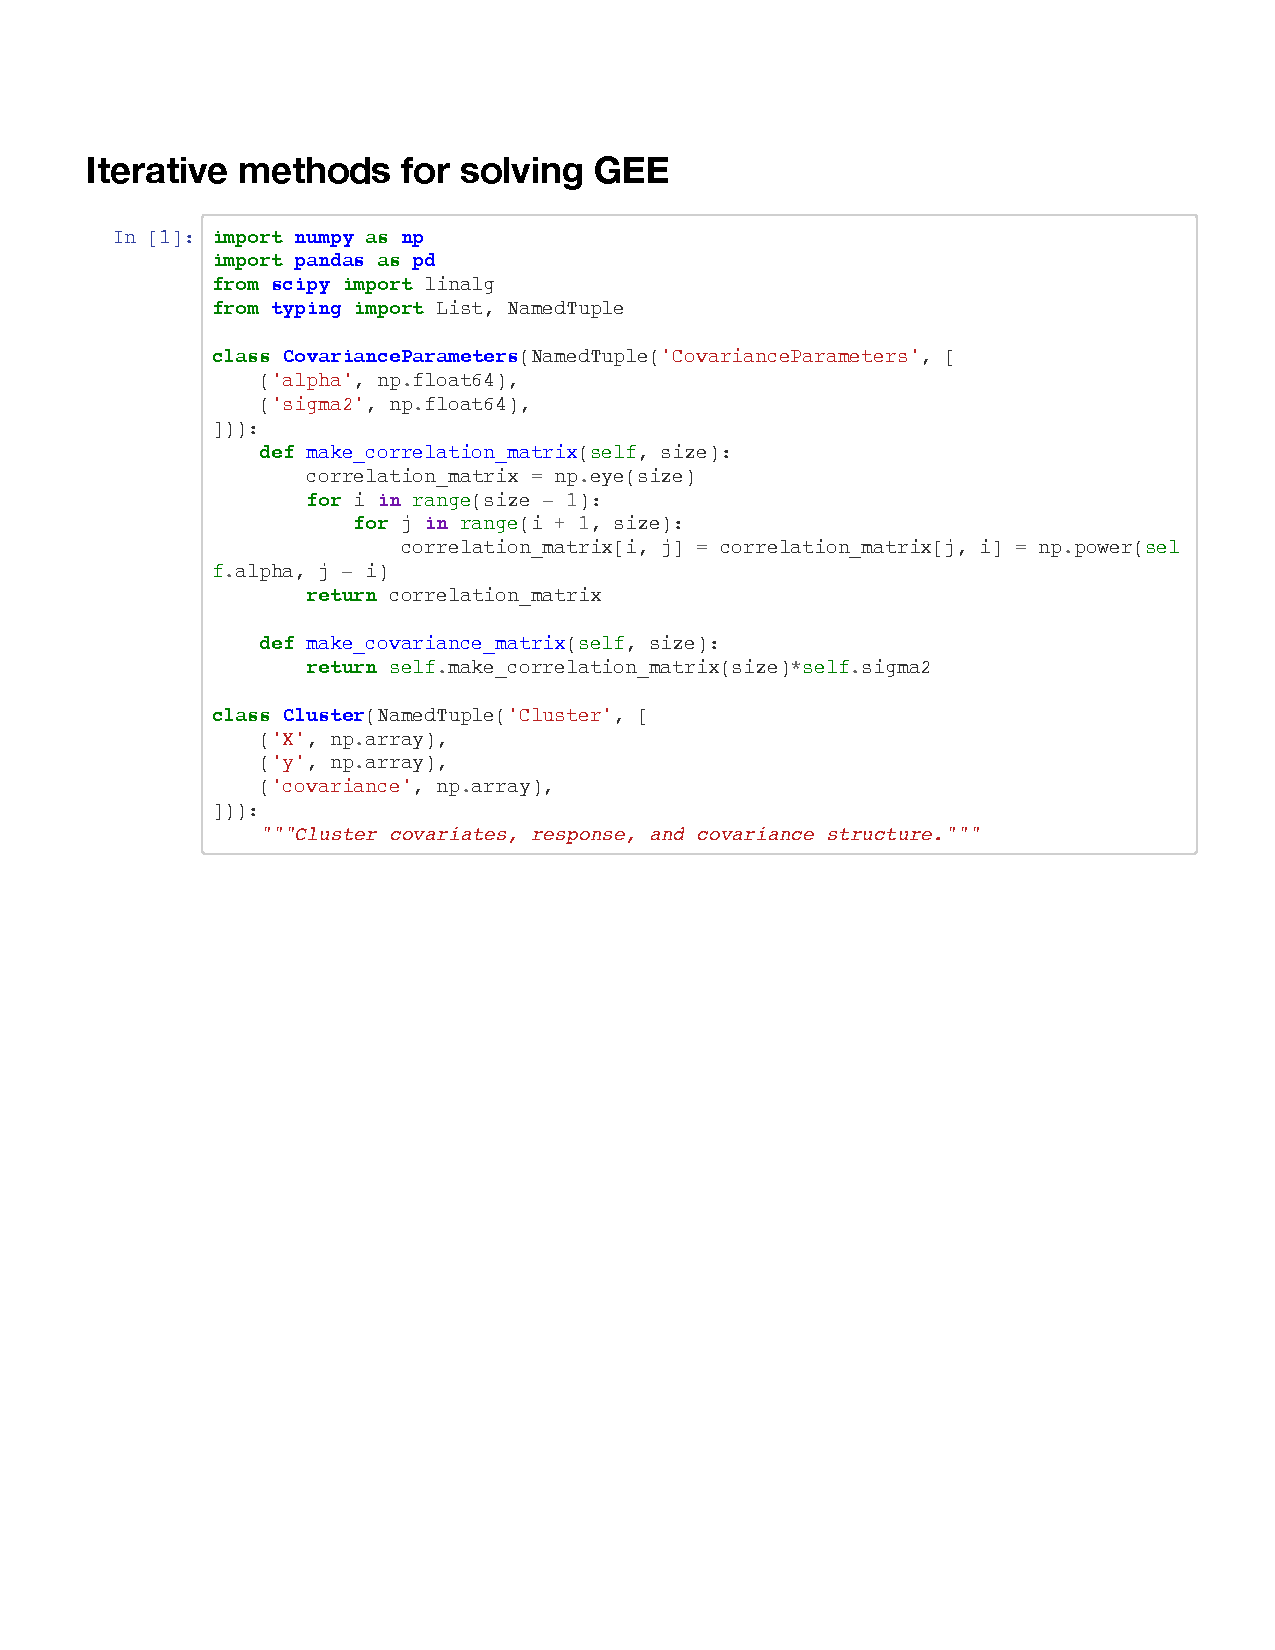
\includepdf[pages=-]{iterative_gee_dental.pdf}

\end{document}